% !TeX spellcheck = <none>
\documentclass[a4paper,12pt,onecolumn,oneside]{article}
\usepackage[UTF8]{ctex}
\usepackage{booktabs}
\usepackage{graphicx} % 用于插入图片
\usepackage{amsmath} % 数学公式
\usepackage{hyperref} % 超链接
\usepackage{caption} % 图片标题
\usepackage{subcaption} % 子图片
\usepackage{geometry}
\geometry{a4paper,scale=0.8}
\usepackage{titlesec}
\titleformat{\section}
{\normalfont\Large\bfseries\centering}{\thesection}{1em}{}
\usepackage{tabularray}
\UseTblrLibrary{diagbox}
\usepackage{subcaption}
\usepackage[table]{xcolor}
\usepackage{colortbl}
\usepackage{listings}
\usepackage{float}
\usepackage{setspace}



\title{乳腺癌数据集上的决策树算法}
\author{第十组}
\date{\today}

\begin{document}
	\maketitle
\begin{abstract}
	乳腺癌一直是致使女性死亡的主要原因之一,因此通过某些生理特性及时判断肿瘤性质以提早发现提早治疗显得尤为重要。
	
	本文通过在威斯康乳腺癌数据集运行决策树算法以实现对肿瘤性质的分类。在运行决策树算法时,我们分别采取选取特征进行不剪枝、预剪枝与后剪枝方法并对上述决策树算法效果进行对比,得出结论为不剪枝所展现出的效果最佳。并且,我们将最优决策树算法与上次报告的其他算法效果进行对比分析,发现决策树算法的表现较差,综合多个评价指标看,KNN算法表现最稳定且效果也很好。针对此结论,我们进行讨论后提出自己的解释。
	
	针对以上分析过程,我们在最后进行了总结,并对模型可能存在的问题进行反思以发现可改进之处。
	
	\textbf{关键词:} 决策树,剪枝,对比分析
	
\end{abstract}
\newpage
\begin{spacing}{1.2}
\tableofcontents
\end{spacing}
\newpage
\section{数据集及任务}
\subsection{数据集描述}
乳腺癌是女性恶性肿瘤里发病率最高的一种,在我国,乳腺癌的发病率为每十万人中大概有22例左右,而且我国乳腺癌患者在逐年增加。为了探究乳腺癌的影响因素,我们选择了威斯康星乳腺癌数据集。该数据集来源于威斯康辛大学关于乳腺癌的相关诊断,展示了良性肿瘤、恶性肿瘤的诊断结果与某些细胞特征的相关性。通过建立模型可以协助医生诊断患者的肿瘤状态,提升诊断的效率,减少漏诊和误诊,进而提升乳腺癌患者的生存率与治愈率。本数据集包含样本编号、块状厚度、细胞大小的均匀性等11个特征的699条数据,具体数据说明如表\ref{tab:dataset}所示。
\begin{table}[h]
	\centering
	\caption{数据说明表}
	\label{tab:dataset}
	\begin{tblr}{
			cells = {c},
			cell{4}{2} = {r=9}{},
			cell{4}{3} = {r=9}{},
			cell{4}{4} = {r=9}{},
			hline{1,13} = {-}{0.08em},
			hline{2} = {-}{0.05em},
		}
		变量名称                        & 变量类型  & 取值范围 & 变量分类 & 备注            \\
		Class                       & 响应变量  & 0/1  & 离散型  & 0:良性肿瘤~1:恶性肿瘤 \\
		Sample code number          & ——    & ——   & ——   & 样本编号          \\
		Clump Thickness             & 解释变量~ & 1-10 & 连续型  & 块状厚度          \\
		Uniformity of Cell Size     &       &      &      & 细胞大小的均匀性      \\
		Uniformity of Cell Shape    &       &      &      & 细胞形状的均匀性      \\
		Marginal Adhesion           &       &      &      & 边缘粘附力         \\
		Single Epithelial Cell Size &       &      &      & 单个上皮细胞大小      \\
		Bare Nuclei                 &       &      &      & 裸核            \\
		Bland Chromatin             &       &      &      & 淡染色质          \\
		Normal Nucleoli             &       &      &      & 正常核仁          \\
		Mitoses                     &       &      &      & 有丝分裂          
	\end{tblr}
\end{table}


\subsection{我们的任务}
\begin{enumerate}
	\item 进行数据预处理,并对数据进行简单的描述性统计分析以初步了解数据特征。
	\item 建立多个评价指标,以评价模型优劣。
	\item 建立两个不剪枝决策树模型,其中一个选取所有变量,另一个删除相关性较高的变量。对两棵决策树进行描述,并根据评价指标,对比两颗决策树的优劣,选出二者中较优的决策树做后续建模。
	\item 对所选出的决策树进行预剪枝和后剪枝处理,生成新的两棵决策树,并进行描述。根据评价指标,对比不剪枝、预剪枝、后剪枝的三棵决策树,并选出最优决策树模型。
	\item 根据评价指标对比最优决策树模型与最优分类算法模型。
	\item 对模型效果进行评价总结,并思考可改进之处。
\end{enumerate}
\subsection{主要函数说明}
\paragraph{基尼系数} 
	基尼指数反映了从数据集中随机抽取两个样本,其类别标记不一致的概率,是特征选择的指标之一。基尼指数定义如下: 
	\begin{equation*}
		Gini(p) = 1 - \sum_{i=1}^{c} p_i^2
	\end{equation*}
	其中,$p$ 是样本集合中属于类别 $i$ 的样本所占的比例,$c$ 是类别的个数。在特征选择过程中,计算每个特征的基尼指数,并选择具有最小基尼指数的特征作为当前节点的判断特征。
\paragraph{GridSearchCV() 函数}
	参数搜索函数,通过在参数空间中的组合进行交叉验证,找到最佳参数配置,最后打印输出模型的最佳评分和最佳参数。
\lstset{language=Python}
\lstset{frame=lines}
\lstset{caption={预剪枝最佳参数搜索}}
\lstset{basicstyle=\footnotesize}
\begin{lstlisting}
	def find_best_param():
	clf = tree.DecisionTreeClassifier(random_state=0)
	param_test = {
		'max_depth': range(1, 10, 1),
		'min_samples_leaf': range(1, 10, 1),
		'random_state': range(0, 100, 5),
		'min_samples_split': range(5, 20, 3),
		'splitter': ('best', 'random'),
		'criterion': ('gini', 'entropy')
	}
	gsearch = GridSearchCV(
	estimator=clf, 
	param_grid=param_test, 
	scoring=None, 
	n_jobs=-1, 
	cv=5, 
	verbose=0
	)
	gsearch.fit(X_train, y_train)
	print(gsearch.best_score_)
	print(gsearch.best_params_)
\end{lstlisting}
\newpage
\section{实验设置}
\vspace{-\baselineskip}
\subsection{预处理}
\subsubsection{缺失值处理}
在进行分类任务之前,我们对威斯康星乳腺癌数据集进行了预处理。具体而言,首先,根据 UCI Machine Learning Repository 关于该数据集的文档说明,数据集中共含有16个缺失值,以 "?" 填补。我们首先以舍入后均值替换这些缺失值。接下来,删除与分类任务无关的 id 号列。
\lstset{language=Python}
\lstset{frame=lines}
\lstset{caption={预处理}}
\lstset{label={lst:code_direct}}
\lstset{basicstyle=\footnotesize}
\begin{lstlisting}
	df = pd.read_csv("breast-cancer-wisconsin.csv", na_values=["?"])
	df = df.fillna(round(df.mean(), 0))
	data = df.iloc[:, 1:]
\end{lstlisting}
\subsubsection{可视化}
此后进行数据可视化。首先观察样本是否平衡,按照肿瘤细胞的良性和恶性分类绘制直方图,如图\ref{fig:hist2}所示。\par
%\begin{figure}[h]
%	\centering
%	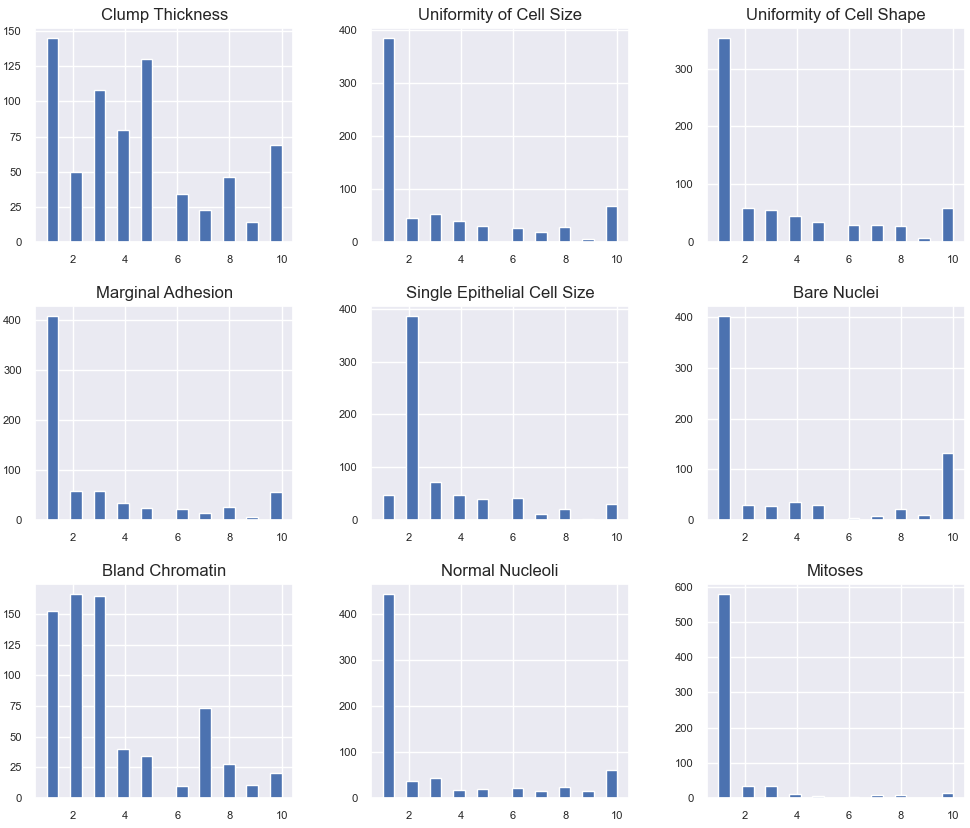
\includegraphics[width=0.75\textwidth]{res3/hist1.png}
%	\caption{样本直方图}
%	\label{fig:hist1}
%\end{figure}
\begin{figure}[H]
	\centering
	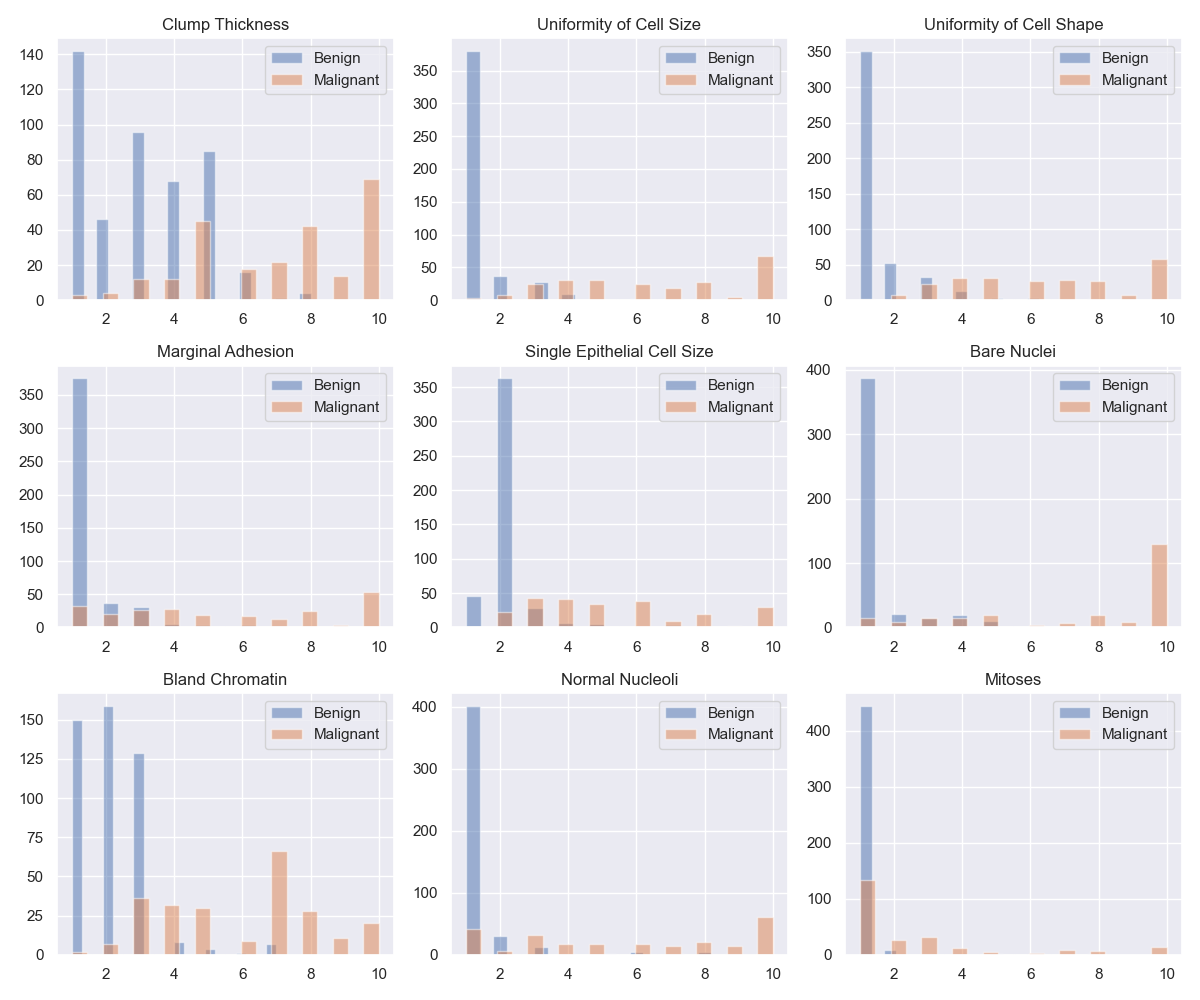
\includegraphics[width=0.8\textwidth]{res3/hist2.png}
	\caption{按照Class分类的样本直方图}
	\label{fig:hist2}
\end{figure}
由上述直方图可看出,肿瘤块状厚度为1的数量最多,且根据条状颜色分布可知,良性肿瘤的块状厚度偏小,而恶行肿瘤的块状厚度偏大;肿瘤细胞大小均匀性为1的数量最多,细胞大小为2—10的数量几乎相等。且根据条状颜色分布可知,良性肿瘤的细胞大小的均匀性集中分布于1,而恶性肿瘤的细胞大小均匀性几乎均匀分布于3-10;观察其他特征的分布可发现,其与上述特征的分布近似相同,总结来看,良性肿瘤的特征均偏低,且分布集中,而恶性肿瘤的特征偏低,且分布近似均匀。且从样本平衡性来看,除肿瘤块状厚度的样本分布较为均匀外,其余特征的样本分布集中分布于取值较低的特征处,且良性肿瘤样本数远大于恶性肿瘤样本数,即样本均衡性较差。\par 
\begin{figure}[H]
	\centering
	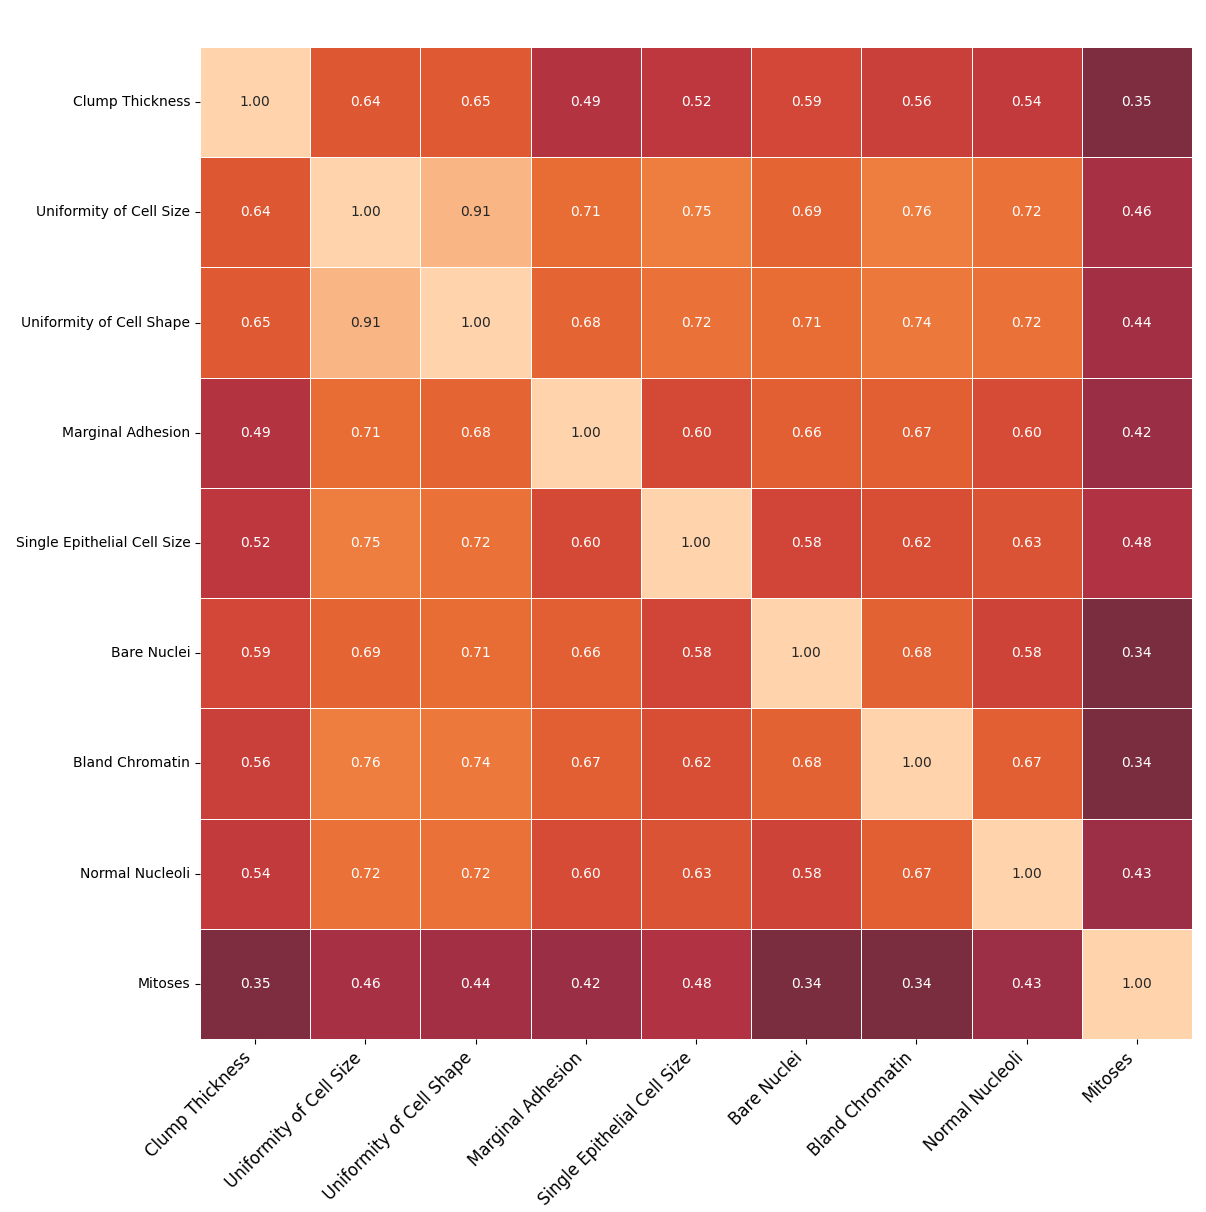
\includegraphics[width=0.9\textwidth]{res3/heatmap.png}
	\caption{相关性热力图}
	\label{fig:heatmap}
\end{figure}
分析九个自变量的相关性情况,如图\ref{fig:heatmap}所示。可以观察到,自变量之间的相关性比较高。因此,在之后的建模过程中,我们考虑尝试通过删除相关性较高的特征来进行数据降维,具体的工作在 \ref{bujianzhi} 中进行。
\subsection{评价指标}
在这一部分中,主要对所选择的模型评价标准参数进行说明。本次共选择五种评价标准进行评价,分别为 Precision、Recall、F1-Score、Maro Avg 和 Weighted Avg。分类器的预测结果可以分为四种情况:
\begin{enumerate}
	\item 真正例(True Positive,TP):分类器将一个实际为正例的样本正确地预测为正例。
	\item 真反例(True Negative,TN):分类器将一个实际为反例的样本正确地预测为反例。
	\item 假正例(False Positive,FP):分类器将一个实际为反例的样本错误地预测为正例。
	\item 假反例(False Negative,FN):分类器将一个实际为正例的样本错误地预测为反例。
\end{enumerate}

精确率 Precision 表示分类器预测为正例的样本中有多少是真正例,定义为
\begin{equation*}
	Precision = \frac{TP}{TP + FP}
\end{equation*}
\par 召回率 Recall 表示真正例中有多少被分类器正确地预测出来了,定义为
\begin{equation*}
	Recall = \frac{TP}{TP + FN}
\end{equation*}
\par 二者的区别在于精确率的分母是预测到的正类,它的提出是让模型的现有预测结果尽可能不出错,即宁愿漏检,也不能让现有的预测有错。而召回率的分母是原本的正类,它的提出是让模型预测到所有想被预测到的样本,即就算多预测一些错的,也能接受。\par
F1-Score 综合了精确率和召回率,是二者的调和平均数,定义为
\begin{equation*}
	\text{F1-Score} = 2\cdot\frac{Precision\times Recall}{Precision+Recall} = \frac{TP}{TP+\frac{1}{2}(FP+FN)}
\end{equation*}
宏平均 Maro Avg 定义为 benign 和 malignant 的 Precision 或 Recall 或 F1-Score 的算数平均值。加权平均 Weighted Avg 的定义为用每一个类别(benign和malignant)的样本数量在所有类别的样本总数的占比作为权重,然后计算 Precision 或 Recall 或 F1-Score 的加权平均值。
\clearpage
\section{决策树算法}
\subsection{算法原理和基本流程}
	决策树是一种基本的机器学习算法,用于解决分类和回归问题。它通过构建树形结构来对数据进行决策。

	决策树由节点和边组成,每个节点表示对某个特征的判断,每个边表示不同的特征取值和判断结果之间的关系。树的根节点代表最初的判断特征,叶节点代表最终的分类或回归结果。

	决策树的构建过程可以分为两个主要步骤:特征选择和树的生成。

	特征选择的目标是确定在每个节点上最优的判断特征,常用的特征选择指标有信息增益(Information Gain)、增益率(Gain Ratio)和基尼指数(Gini Index)。其中,基尼指数是最常用的特征选择指标之一。
	
	树的生成是通过递归地构建节点和边来完成的。在每个节点上,根据判断特征的取值,将数据集划分为不同的子集。然后,对每个子集递归地执行特征选择和树的生成过程,直到满足停止条件(例如达到最大深度、样本数小于阈值等)为止。
	
	决策树生成完毕后,可以使用它来进行分类或回归预测。对于分类问题,通过从根节点开始,根据判断特征的取值沿着树的路径向下移动,最终到达叶节点,得到分类结果。对于回归问题,叶节点存储的是样本的平均值或其他统计量,预测结果是从根节点到达的叶节点的平均值或其他统计量。

\subsection{不剪枝决策树算法}\label{bujianzhi}
	使用默认参数,在数据集上生成不剪枝的决策树,代码如下所示。
	\lstset{language=Python}
	\lstset{frame=lines}
	\lstset{caption={不剪枝决策树}}
	\lstset{basicstyle=\footnotesize}
	\begin{lstlisting}
	def generate_original_tree():
		clf = tree.DecisionTreeClassifier(random_state=75)
		clf = clf.fit(X_train, y_train)
		y_pred = clf.predict(X_test)
		y_true = y_test
		report = classification_report(y_true, y_pred)
		print(report)
		accuracy = accuracy_score(y_true, y_pred)
		print("Accuracy: {:.4f}".format(accuracy))
		return clf
	\end{lstlisting}
	生成的决策树如图 \ref{fig:tree0} 所示。
	\begin{figure}[H]
		\centering
		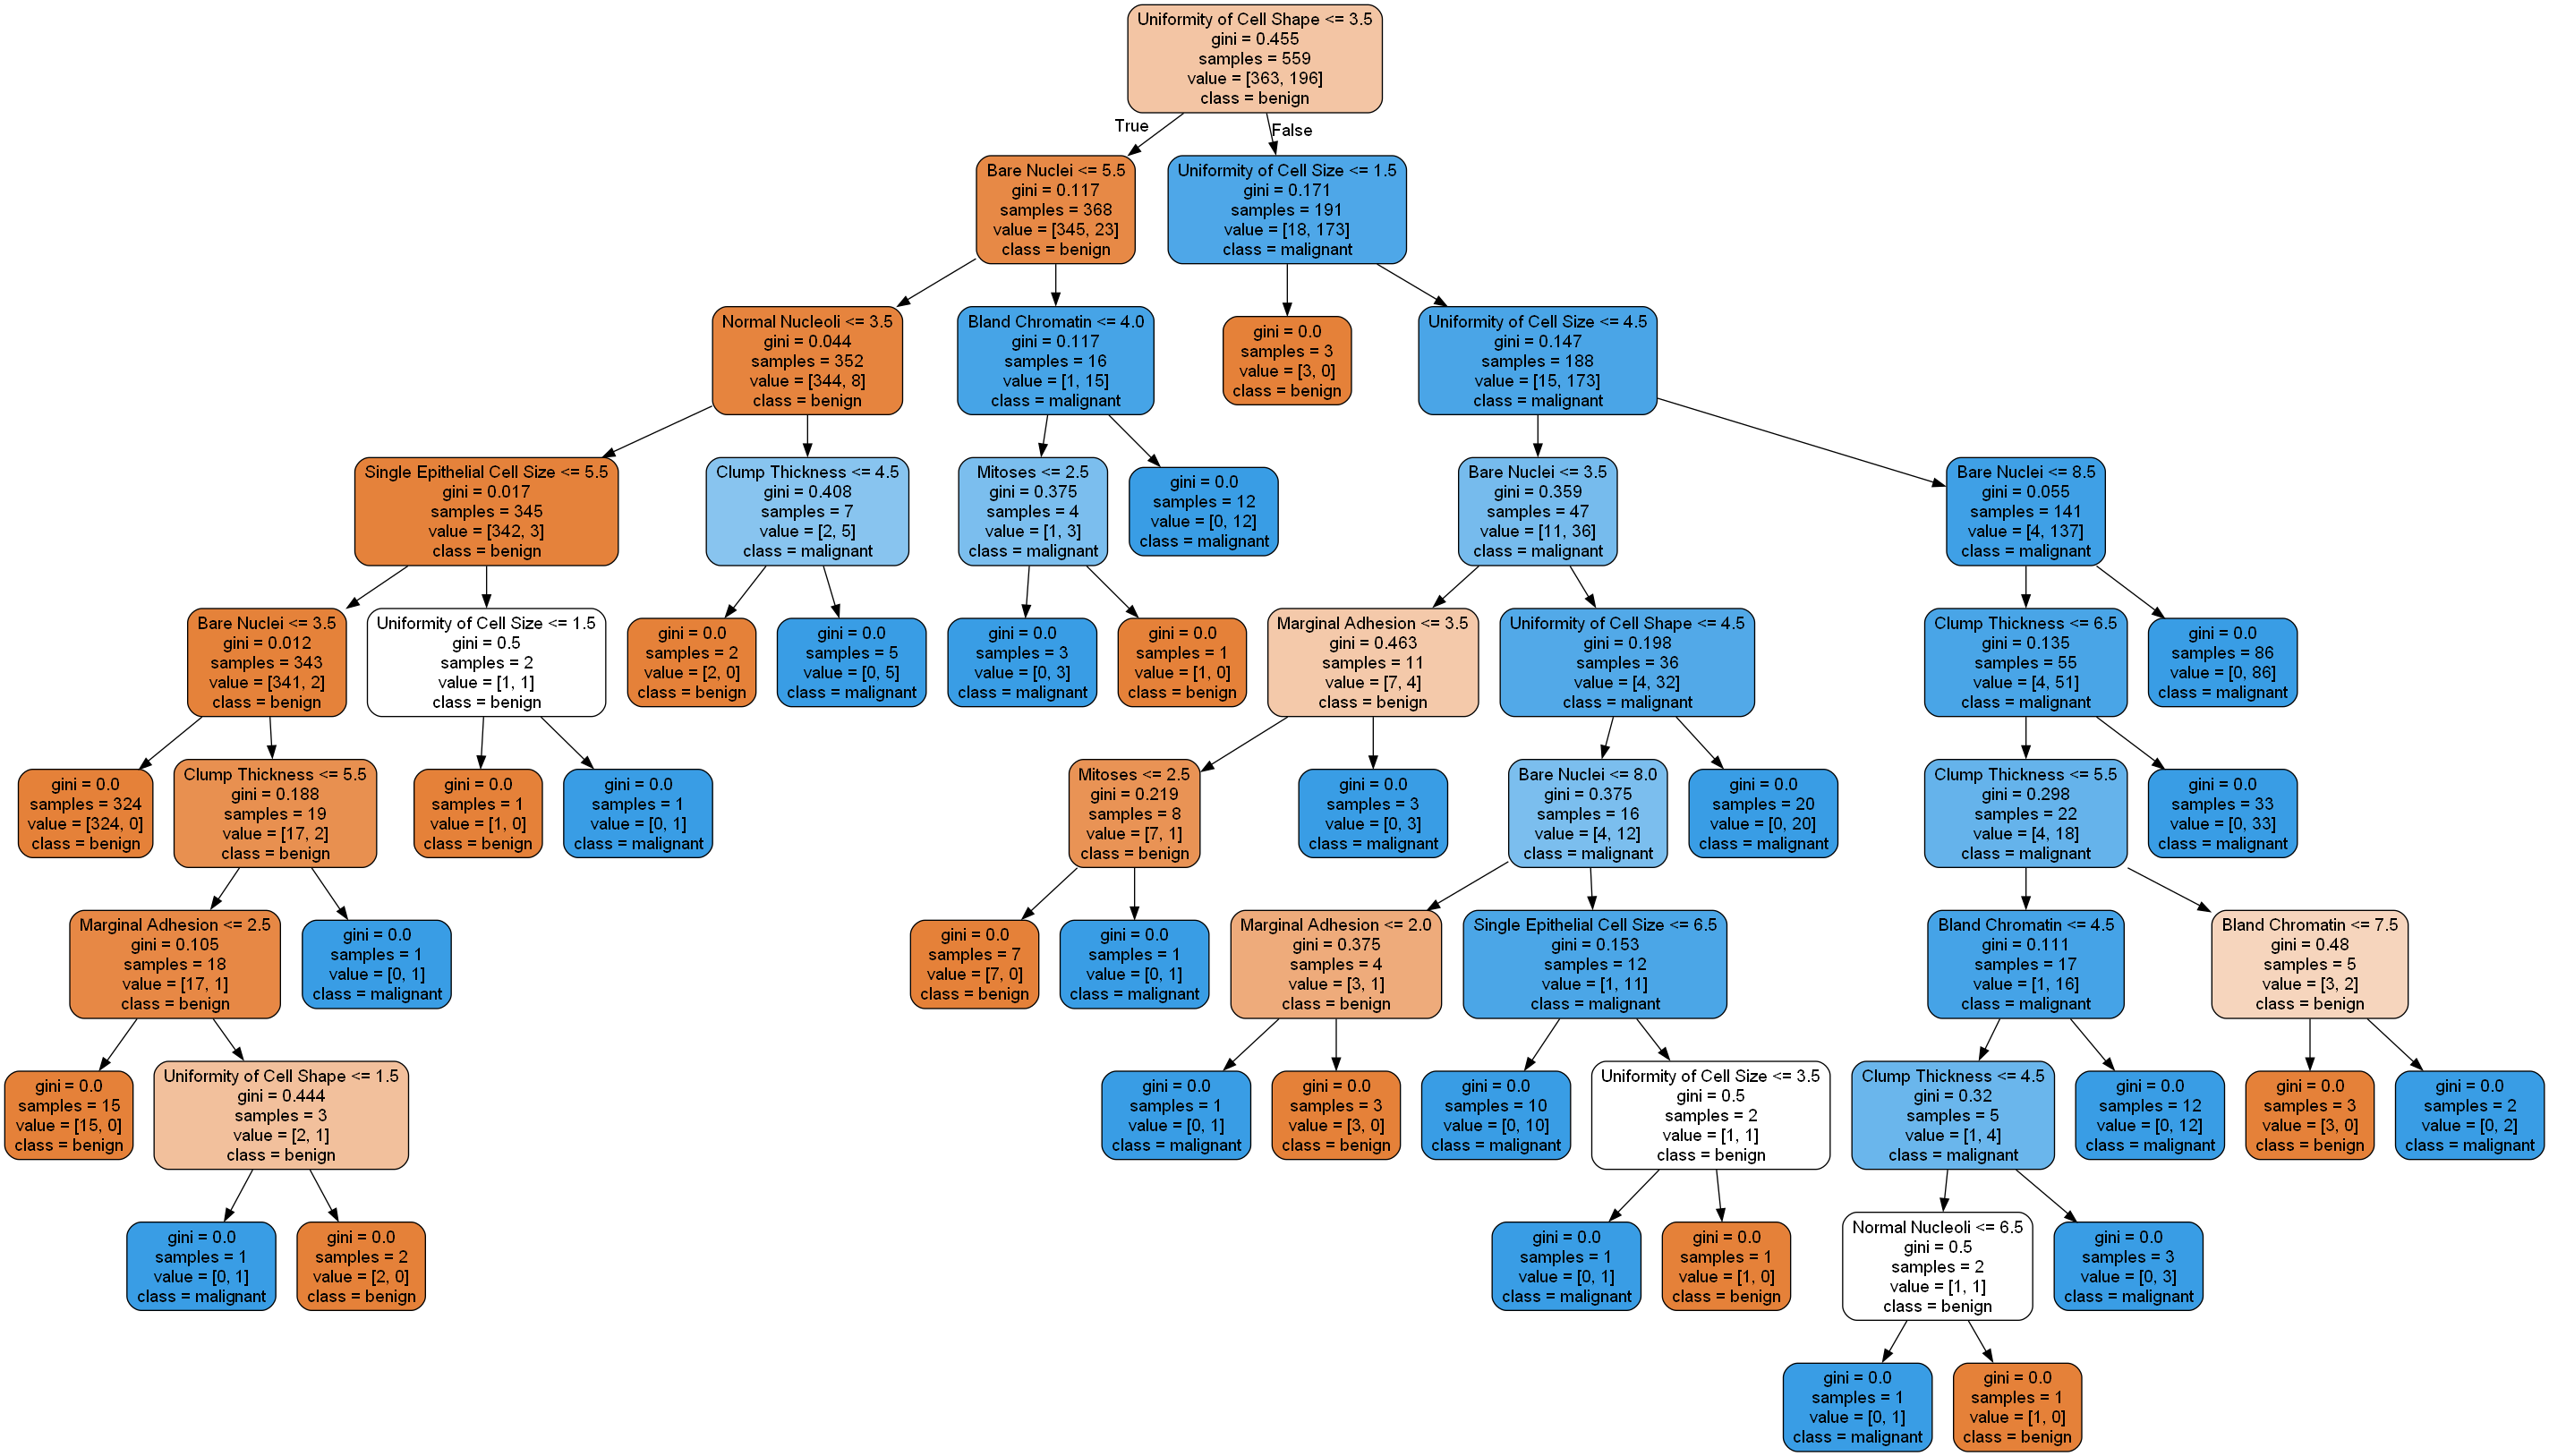
\includegraphics[width=0.9\textwidth]{res3/trees/tree_0.png}
		\caption{不剪枝决策树}
		\label{fig:tree0}
	\end{figure}
	不剪枝决策树的 accuracy 为 95.71\%,对于良性类别,其 precision、recall、f1-score 都比较高,分别为 0.96、0.98、0.97,这表明不剪枝决策树在识别良性肿瘤的时候非常准确并且有很好的召回率。对于恶性类别,precision 指标也很高,为 0.95,但 recall 和 f1-score 指标相对较低,且略低于良性类别,这意味着不剪枝决策树在测恶性肿瘤细胞的时候准确率较低。总体来说,分类器在分类任务中表现良好,但同时也可以发现该模型复杂度太高,过拟合问题较严重。
	\begin{table}[H]
		\centering
		\begin{tabular}{lccc}
			\toprule
			\textbf{Class} & \textbf{Precision} & \textbf{Recall} & \textbf{F1-Score} \\
			\midrule
			\textbf{benign} & 0.96 & 0.98 & 0.97 \\
			\textbf{malignant} & 0.95 & 0.91 & 0.93 \\
			\midrule
			\textbf{Macro Avg} & 0.96 & 0.95 & 0.95 \\
			\textbf{Weighted Avg} & 0.96 & 0.96 & 0.96 \\
			\bottomrule
		\end{tabular}
		\caption{不剪枝决策树性能}
		\label{tbl:origin}
	\end{table}
	其特征的贡献度如图\ref{fig:oringinimportance}所示。可以看出,贡献率最大的变量是“Uniformity of Cell Shape”,其贡献率达到了 70\% 左右。其次是“Bare Nuclei”,其贡献率达到了 15\% 左右。而其余特征的贡献度几乎都是微乎其微的。这一现象表明,特征“Uniformity of Cell Shape”和“Bare Nuclei”可能在建模过程中具有更强的相关性或预测能力,而其他特征可能在模型中没有得到充分利用,或者与目标变量之间的关系较弱。(事实上,在后剪枝的过程中我们认为的最佳决策树最终也只保留了这两个特征,参见 \ref{houjianzhi}。)
	\begin{figure}[H]
		\centering
		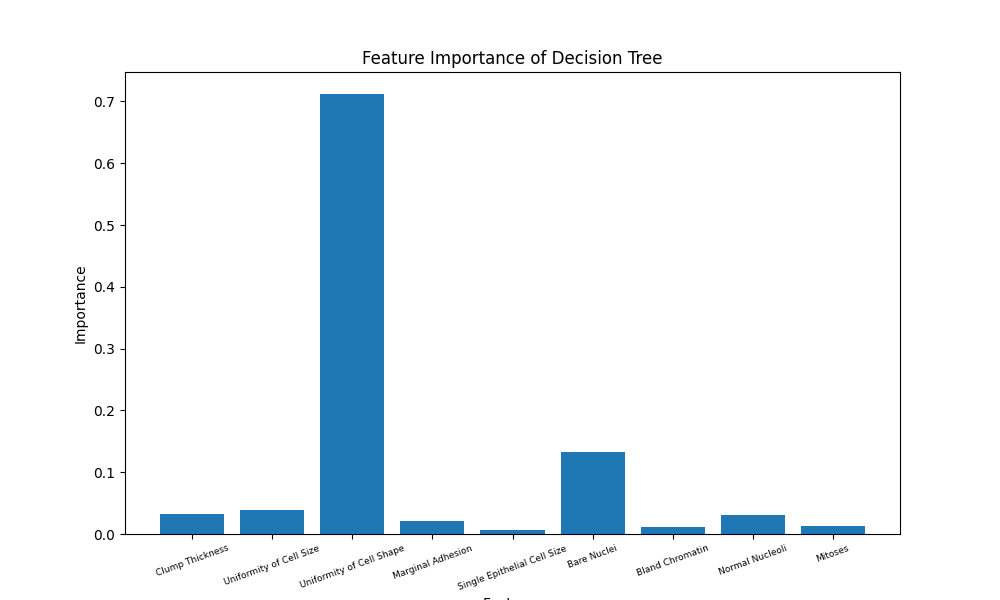
\includegraphics[width=0.9\textwidth]{res3/origin_importance.png}
		\caption{不剪枝决策树特征贡献度}
		\label{fig:oringinimportance}
	\end{figure}
	
	
	由上图可以看出保留全部变量的决策树太过复杂,存在过拟合现象较严重。因此下面考虑依据相关性剔除部分变量以减少该问题。由图2热力图可以看出,变量 Uniformity of Cell shape 与 Bland Chromatin 这两个变量与其他变量的相关性均很强,因此考虑将这两个变量剔除后重新生成不剪枝决策树,结果如下图。
	\begin{figure}[H]
		\centering
		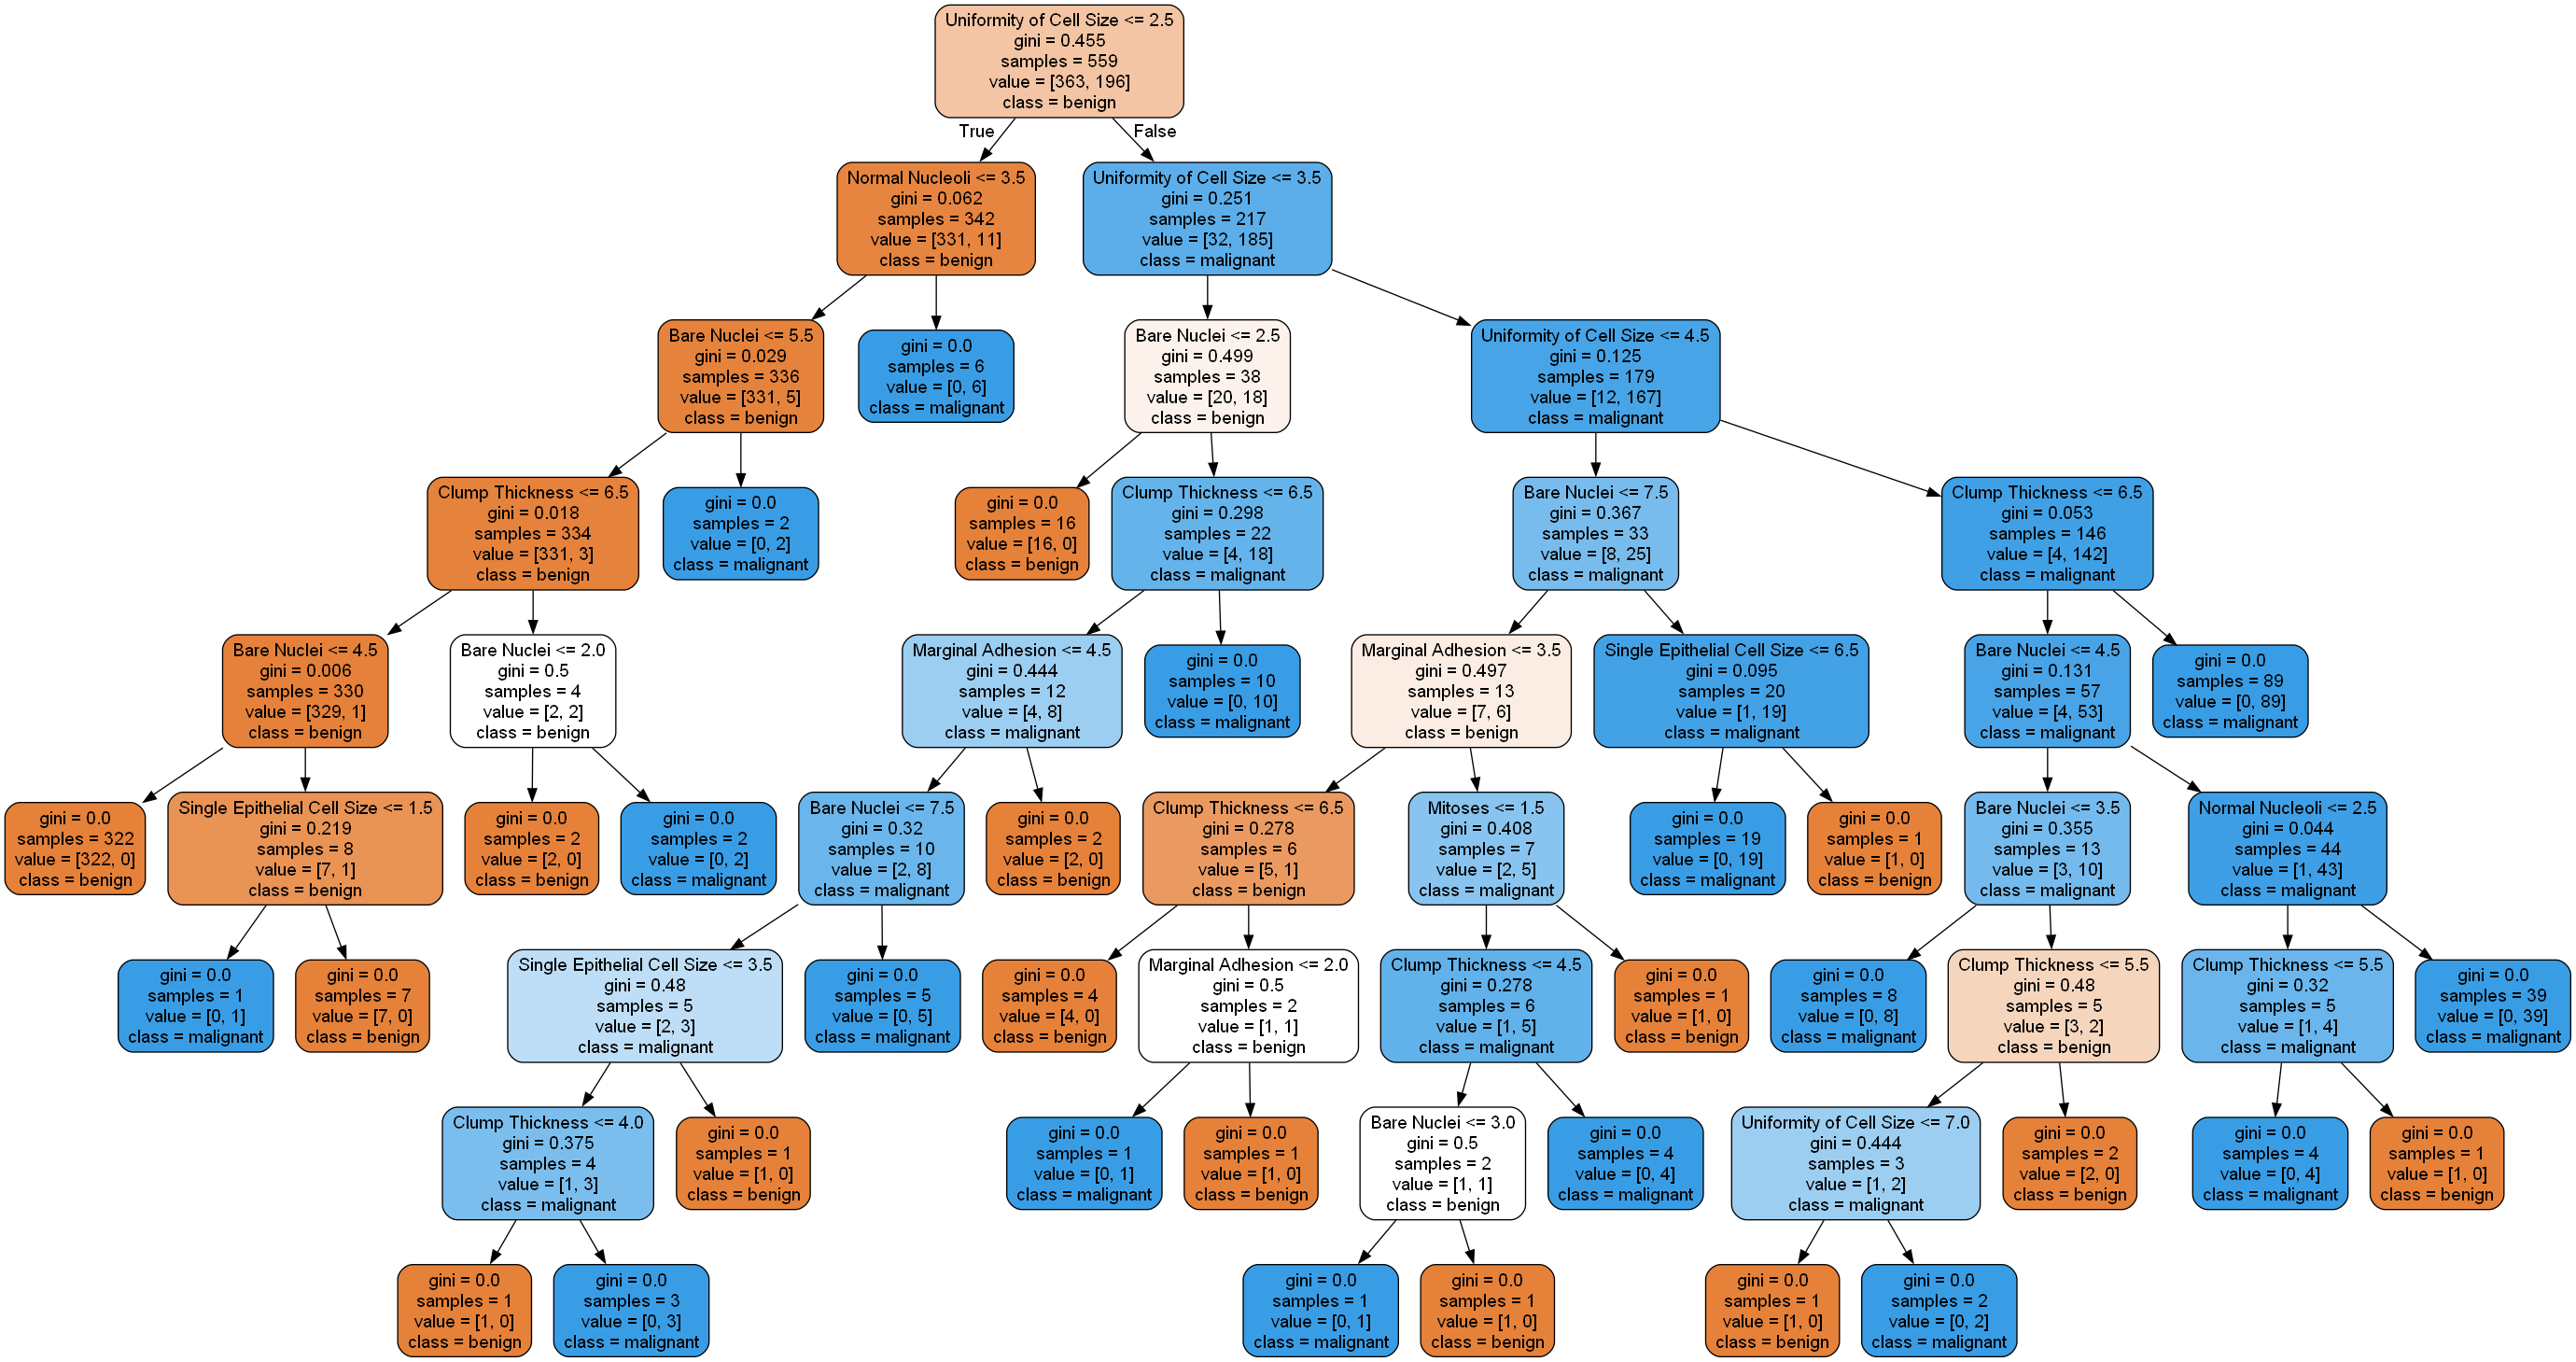
\includegraphics[width=0.9\textwidth]{res3/trees/tree_2.png}
		\caption{删除两变量后不剪枝决策树}
		\label{fig:treecor}
	\end{figure}
	其 Accuracy 为 93.57\%,低于保留全部变量的决策树效果。此外,对比两棵树可以发现决策树变化不大,模型复杂度变化不明显,因此综合来看,不剪枝决策树仍存在较严重的过拟合问题,后续应针对此问题提出解决方法。
\section{剪枝策略及其应用}
	决策树算法具有易于理解和解释、能够处理数值型和类别型数据、能够处理缺失数据等优点。然而,它也存在容易过拟合、对输入数据的小变化敏感等缺点。为了解决这些问题,可以使用剪枝方法。
\subsection{预剪枝}
	决策树算法中的预剪枝(pre-pruning)是一种用于减少决策树过拟合的技术。过拟合指的是决策树过于复杂,过度适应训练数据,导致在未见过的数据上表现不佳。
	
	预剪枝是在构建决策树的过程中,在每个节点进行划分之前进行判断,以确定是否应该终止节点的划分。它通过一些预定义的条件来决定是否进行划分,从而限制了决策树的生长。
	
	一些常用的预剪枝技术包括:
	\begin{enumerate}
		\item 最大深度限制:限制决策树的最大深度。当达到指定的深度时,停止树的进一步生长,将当前节点标记为叶节点。
		\item 叶节点样本数限制:设置一个阈值,当节点上的样本数小于该阈值时,停止树的进一步生长,将当前节点标记为叶节点。
		\item 不纯度减少阈值:定义一个阈值,当节点上的不纯度减少量小于该阈值时,停止树的进一步生长,将当前节点标记为叶节点。
		\item 提前终止条件:在训练过程中监测验证集的性能,如果验证集的性能没有进一步提升,则停止树的生长。
	\end{enumerate}
	在实践中,我们选择网格搜索进行调参,从而达到预剪枝的目的,具体而言,我们将生成决策树的参数设置在一定范围内,使用 GridSearchCV 函数进行参数搜索,通过在参数空间中的组合进行交叉验证,找到最佳参数配置,最后打印输了模型的最佳评分和最佳参数。这样生成的参数配置被认为是最佳的,因为它们使得模型在交叉验证过程中获得了最好的性能评分。通过使用这些最佳参数来构建决策树模型,可以期望在未见过的数据上获得更好的预测性能。生成的最佳参数组合为:
	\begin{enumerate}
		\item criterion:划分质量的评价准则,这里选择了'gini',即基尼系数。
		\item max\_depth:决策树的最大深度为5,这表示决策树最多可以有5层。
		\item min\_samples\_leaf:叶节点的最小样本数为7,当叶节点的样本数少于7时,不再进行进一步划分。
		\item min\_samples\_split:内部节点分裂所需的最小样本数为5,当节点上的样本数少于5时,不再进行分裂。
		\item random\_state:随机种子为75,用于确保结果的可重复性。
		\item splitter:节点划分的策略为'random',即随机选择划分特征。
	\end{enumerate}
	将以上最佳参数用于生成决策树,代码如下所示。得到的决策树如图 \ref{fig:tree1} 所示。其 Accuracy 为 93.57\%。其余指标如表 \ref{tbl:1} 所示。
	\lstset{language=Python}
	\lstset{frame=lines}
	\lstset{caption={生成预剪枝最佳参数树}}
	\lstset{basicstyle=\footnotesize}
	\begin{lstlisting}
	def best_param_tree():
		clf = tree.DecisionTreeClassifier(
			max_depth=5, 
			min_samples_leaf=7, 
			min_samples_split=5,
			criterion="gini", 
			random_state=75, 
			splitter="random"
			)
		clf = clf.fit(X_train, y_train)
		y_pred = clf.predict(X_test)
		y_true = y_test
		report = classification_report(y_true, y_pred)
		print(report)
		accuracy = accuracy_score(y_true, y_pred)
		print("Accuracy: {:.4f}".format(accuracy))
		return clf
	\end{lstlisting}
		\begin{table}[H]
		\centering
		\begin{tabular}{lccc}
			\toprule
			\textbf{Class} & \textbf{Precision} & \textbf{Recall} & \textbf{F1-Score} \\
			\midrule
			\textbf{benign} & 0.93 & 0.98 & 0.95 \\
			\textbf{malignant} & 0.95 & 0.84 & 0.89 \\
			\midrule
			\textbf{Macro Avg} & 0.94 & 0.91 & 0.92 \\
			\textbf{Weighted Avg} & 0.94 & 0.94 & 0.93 \\
			\bottomrule
		\end{tabular}
		\caption{预剪枝决策树性能}
		\label{tbl:1}
	\end{table}
	\begin{figure}[H]
		\centering
		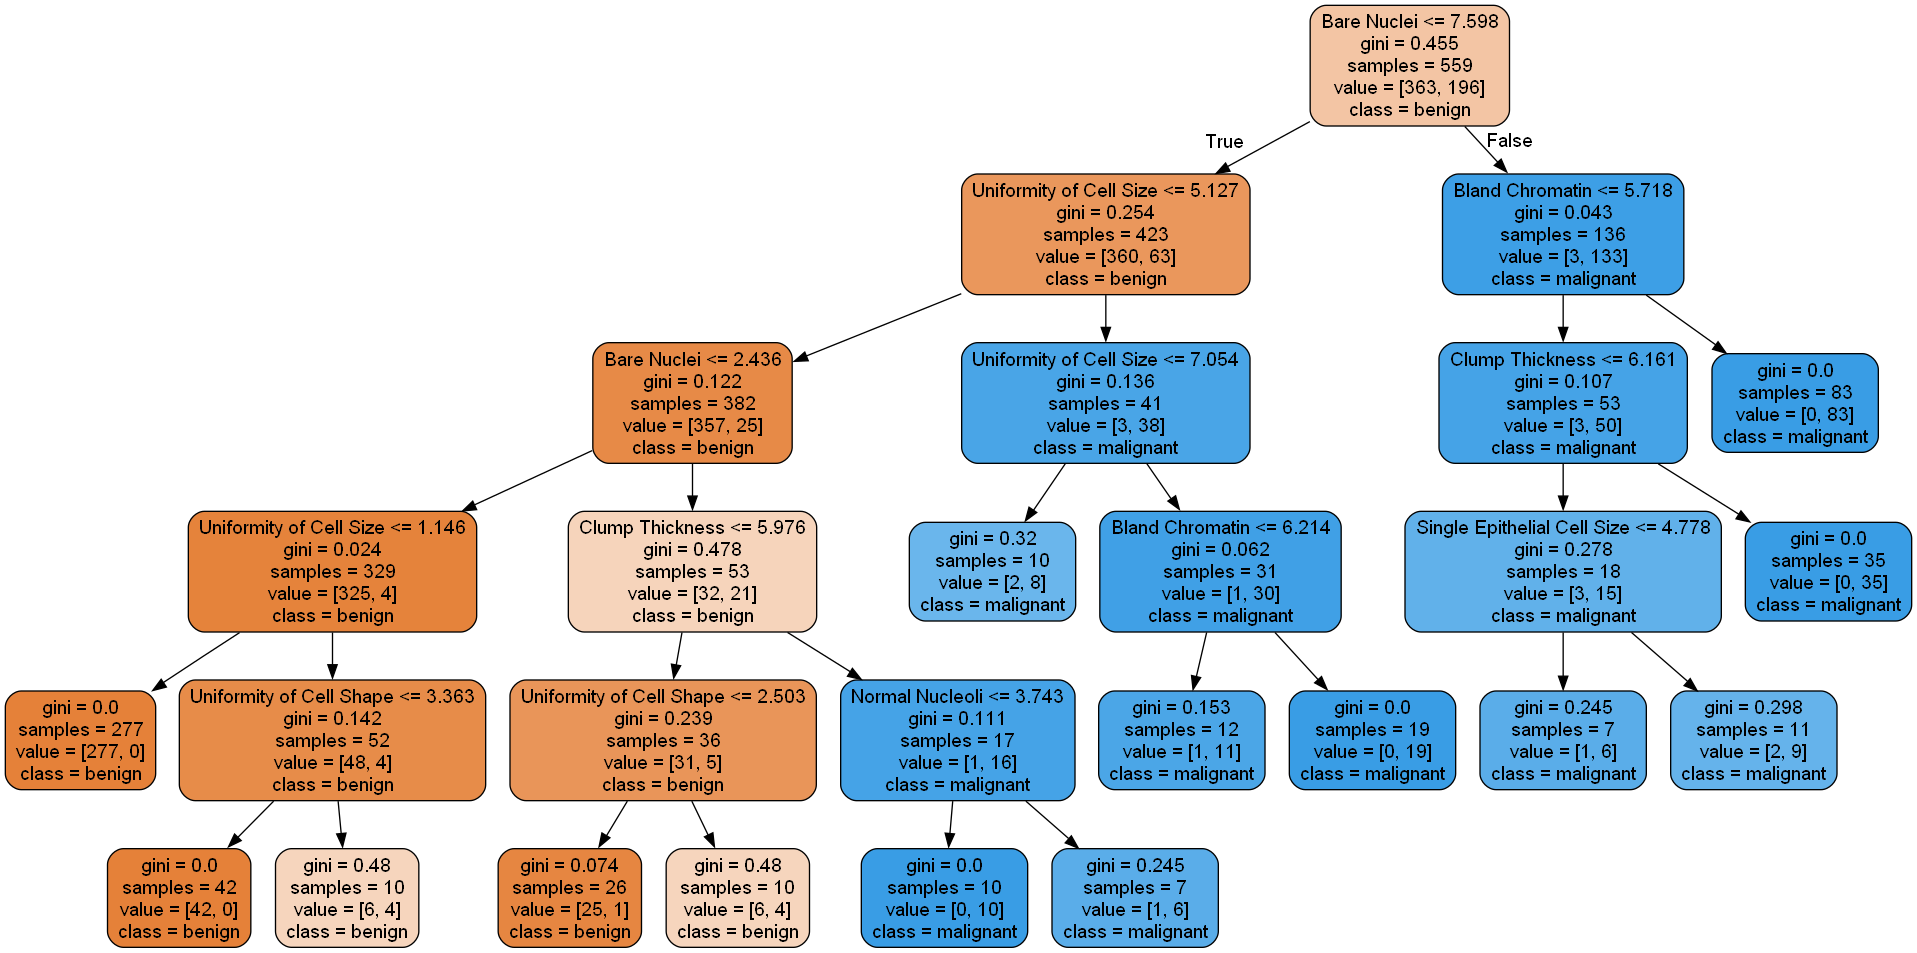
\includegraphics[width=0.9\textwidth]{res3/trees/tree_1.png}
		\caption{预剪枝决策树}
		\label{fig:tree1}
	\end{figure}

	\begin{figure}[H]
		\centering
		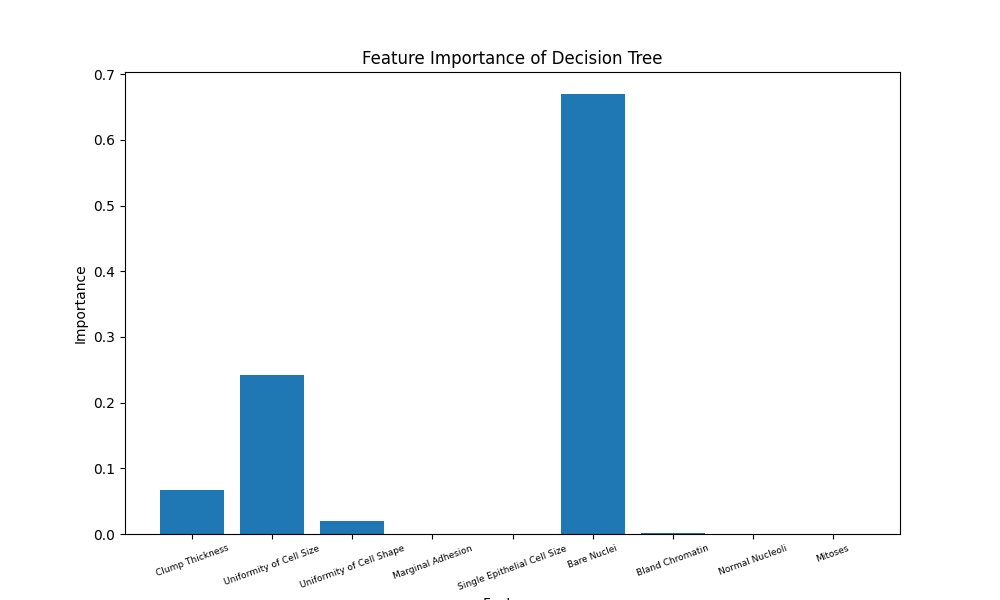
\includegraphics[width=0.9\textwidth]{res3/bestparam_importance.png}
		\caption{预剪枝决策树特征贡献度}
		\label{fig:bestimportance}
	\end{figure}
	
	其特征贡献度如图 \ref{fig:bestimportance} 所示。可以发现,特征贡献度发生了显著的变化。“Bare Nuclei”的贡献度从原先的 15\% 左右增长到了接近 70\%,而原先贡献度最大的特征“Uniformity of Cell shape”的贡献度却变得很低,低于 10\%。这可能是由于这两个特征的相关度较大导致的(事实上,全部9个特征的相关度都很大)。我们通过网格搜索最佳参数确定了剪枝原则后,由图 \ref{fig:tree1} 所示,它选择了“Bare Nuclei”作为节点分裂的最佳候选,这会导致与其相关性高的特征的贡献度下降。除此之外,我们的数据有一定的样本不平衡问题,由于预剪枝更倾向于选择那些对多数类别更具区分性的特征,某些特征在少数类别上的贡献度可能会降低。
	
\subsection{后剪枝}\label{houjianzhi}
	预剪枝可以减少决策树的复杂度,并且能够在一定程度上防止过拟合。然而,由于预剪枝是在构建树的过程中进行判断,可能会导致决策树过于简单,无法充分利用数据的信息。因此,我们也会通过后剪枝(post-pruning)算法来对决策树进行剪枝。
	
	根据CCP(Cost-Complexity Pruning)路径剪树是一种常用的后剪枝算法。它基于决策树节点的CCP值来进行剪枝,CCP值是通过计算每个内部节点的成本复杂度来得到的。
	
	具体的根据CCP路径对决策树进行后剪枝的算法步骤如下:
	
	\begin{enumerate}
		\item 构建完整的决策树,直到每个叶节点都包含同一类别的样本,或无法继续划分为止。
		\item 对每个内部节点,计算其CCP值。CCP值由节点的不纯度和节点的样本数目共同决定。可以使用以下公式计算CCP值:CCP值 = 不纯度减少量 / 节点的样本数目 + $\alpha$。其中,不纯度减少量是每个内部节点的不纯度与其子节点不纯度之差的总和,$\alpha$ 是一个非负参数,用于平衡不纯度减少量和树的复杂度。较大的 $\alpha$ 值倾向于剪去更多的节点,而较小的 $\alpha$ 值倾向于保留更多的节点。
		\item 对于每个非叶节点,计算其CCP值与其子节点的CCP值之和。这个过程从叶节点开始,逐级向上计算。
		\item 构建一个CCP路径,从根节点到每个内部节点,记录下每个内部节点在路径上的CCP值与子节点CCP值之和。
		\item 根据CCP路径中的CCP值,选择具有最小CCP值的节点作为剪枝点。
		\item 剪除选择的剪枝点及其所有子节点,将剪枝点变为叶节点,并将其类别设定为该剪枝点上最频繁的类别。
		\item 重复步骤5和步骤6,直到无法继续剪枝或剪枝后的性能无法提升为止。
	\end{enumerate}
	
	根据CCP路径剪树的算法通过考虑决策树节点的CCP值来选择合适的剪枝点,从而减小模型的复杂度,提高模型的泛化能力。调整 $\alpha$ 参数可以控制剪枝的程度,根据具体问题的特点选择合适的 $\alpha$ 值。一般来说,可以通过交叉验证或其他评估指标来选择最佳的 $\alpha$ 值,以获得在未见过的数据上表现良好的剪枝后的决策树模型。
	
	首先,打印 CCP 路径和不纯度,来判断 $\alpha$ 的取值范围。
	
	\lstset{language=Python}
	\lstset{frame=lines}
	\lstset{caption={查看 CCP 路径和不纯度}}
	\lstset{basicstyle=\footnotesize}
	\begin{lstlisting}
		pruning_path = clf.cost_complexity_pruning_path(X_train, y_train)
		print("ccp_alphas:", pruning_path['ccp_alphas'])
		print("impurities:", pruning_path['impurities'])
		return clf
	\end{lstlisting}
	
	可以选择的alpha值的范围是从0到最大的 ccp\_alpha 值。在我们的结果中,最大的 ccp\_alpha 值为 0.31989666。因此我们令 alpha 值从 0 到 0.31 生成决策树,并打印其不纯度和 Accuracy,代码如下所示,结果如图 \ref{fig:acc} 所示。
	
	\lstset{language=Python}
	\lstset{frame=lines}
	\lstset{caption={查看不同 alpha 值下的不纯度和 Accuracy}}
	\lstset{basicstyle=\footnotesize}
	\begin{lstlisting}
	def find_best_alpha():
		alpha_values = [0.01 * i for i in range(32)]
		accuracies = []
		impurities = []
		
		for alpha in alpha_values:
			clf2, accuracy = ccp_tree(alpha)
			is_leaf = clf2.tree_.children_left == -1
			tree_impurity = (clf2.tree_.impurity[is_leaf] * 
				clf2.tree_.n_node_samples[is_leaf] / 
				len(y_train)).sum()
			accuracies.append(accuracy)
			impurities.append(tree_impurity)
			print(f"Impurity after setting alpha={alpha}:",
				 tree_impurity)
			print("Accuracy: {:.4f}".format(accuracy))
		
		plt.figure(figsize=(10, 6))
		plt.plot(alpha_values, accuracies, marker='o', label='Accuracy')
		plt.plot(alpha_values, impurities, marker='o', label='Impurity')
		plt.xlabel('Alpha')
		plt.ylabel('Value')
		plt.title('Accuracy and Impurity vs Alpha')
		plt.legend()
		plt.show()
	\end{lstlisting}
	\begin{figure}[H]
		\centering
		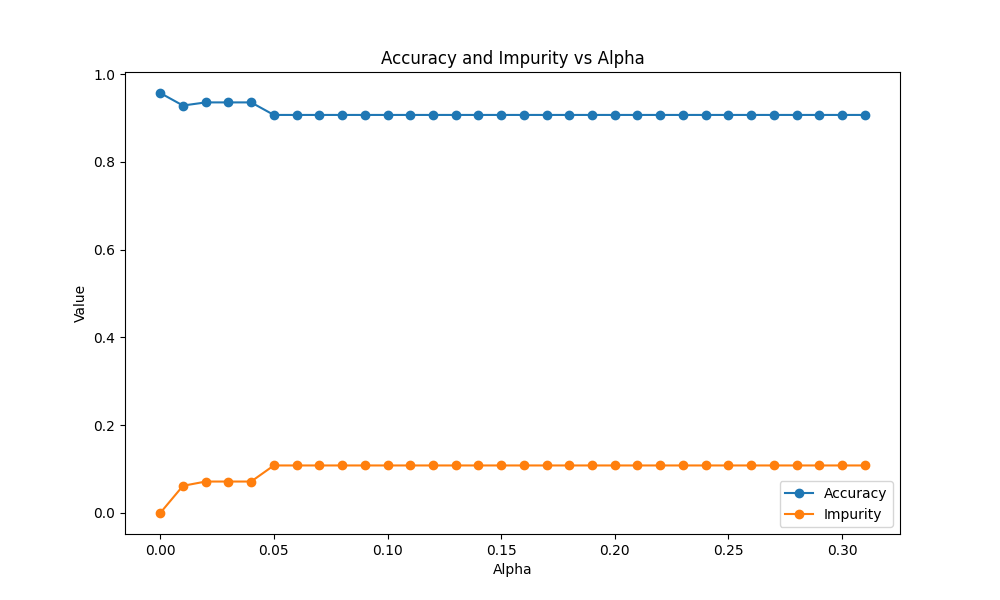
\includegraphics[width=0.9\textwidth]{res3/accimp.png}
		\caption{不同 alpha 值下的不纯度和 Accuracy}
		\label{fig:acc}
	\end{figure}
	$\alpha = 0$ 时为不剪枝决策树。由图可以看出,准确度与不纯度都近似可看作 3 阶阶梯函数,当 $\alpha$ 在 0.02 - 0.04 阶段,不纯度几乎不变而准确度略有上升,当 $\alpha = 0.05$ 时,模型不纯度有较大幅度提高且准确度有较大幅度下跌。因此我们有理由认为当 $\alpha = 0.04$ 时,决策树效果较好。下面输出 $\alpha = 0.04$ 时的决策树模型如图 \ref{fig:tree_0.04} 所示,特征贡献度如图 \ref{fig:tree_0.04_imp} 所示,其余性能如表 \ref{tbl:alpha0.04} 所示。
	\begin{figure}[H]
		\centering
		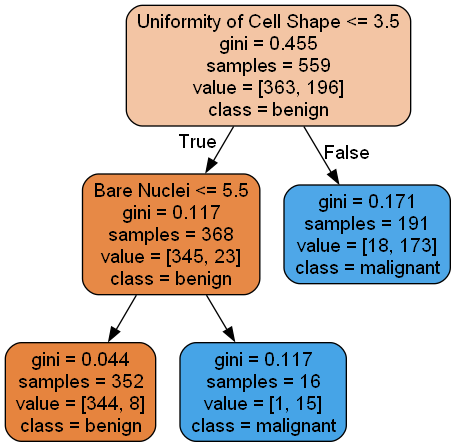
\includegraphics[width=0.4\textwidth]{res3/trees/tree_0.04.png}
		\caption{alpha = 0.04, Impurity = 0.089, Accuracy = 0.9357}
		\label{fig:tree_0.04}
	\end{figure}
	
	\begin{figure}[H]
		\centering
		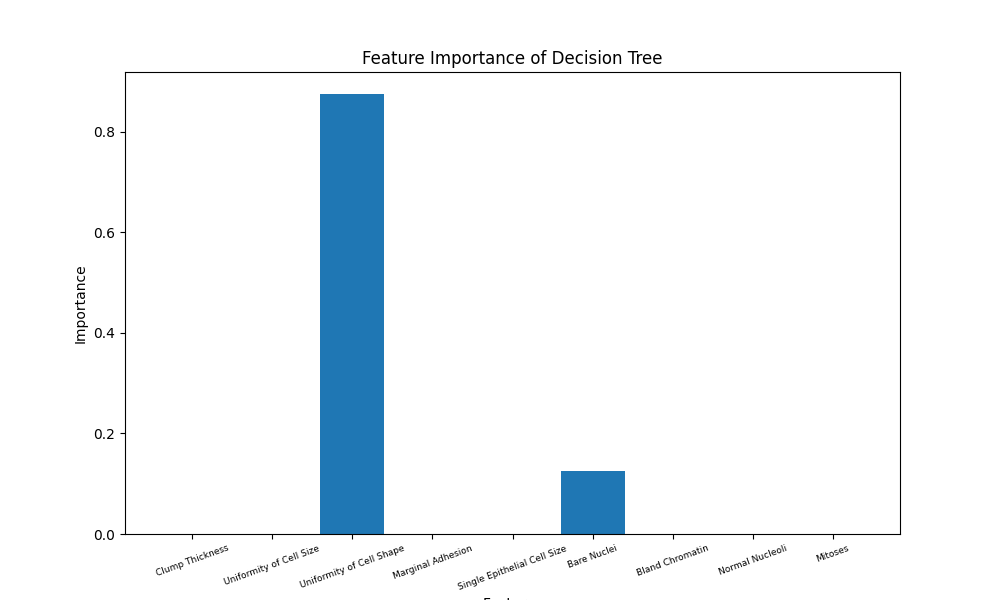
\includegraphics[width=0.9\textwidth]{res3/best_importance.png}
		\caption{alpha = 0.04 的后剪枝决策树特征贡献度}
		\label{fig:tree_0.04_imp}
	\end{figure}
	
	\begin{table}[H]
	\centering
	\begin{tabular}{lccc}
		\toprule
		\textbf{Class} & \textbf{Precision} & \textbf{Recall} & \textbf{F1-Score} \\
		\midrule
		\textbf{benign} & 0.96 & 0.95 & 0.95 \\
		\textbf{malignant} & 0.89 & 0.91 & 0.90 \\
		\midrule
		\textbf{Macro Avg} & 0.92 & 0.93 & 0.93 \\
		\textbf{Weighted Avg} & 0.94 & 0.94 & 0.94 \\
		\bottomrule
	\end{tabular}
	\caption{alpha = 0.04 的后剪枝决策树性能}
	\label{tbl:alpha0.04}
	\end{table}
	
	综合看待决策树算法,可以看到不剪枝决策树树高 9 层,存在较严重的过拟合现象,而利用基尼指数评判准则进行后剪枝后仅保留 3 层,且准确度下降的幅度处于可以接受状态。因此可认为后剪枝效果较好。而预剪枝树高 6 层,复杂程度下降较少且准确度偏低。因此也可以看出后剪枝减轻过拟合现象的效果较好且损失精度较少。综合来看,我们组认为损失精度在可接受范围内,最佳决策树为后剪枝生成的。
	
	\subsection{总结}
	由上述分析可知,我们选取了预剪枝和后剪枝两种策略进行模型精炼。预剪枝树高 6 层,precision 值为 0.93。后剪枝方法中由于选取不同模型复杂度参数可生成不同决策树。通过观察图 \ref{fig:acc} 可知无论从模型准确度还是复杂度看,选取调节参数 $\alpha = 0.04$ 的树都是最合适的。其树高 3 层,仅选取 Uniformity of Cell shape 与 Bare Nuclei 两个结点,且以第一个变量为根节点。准确度为 93.57\%,效果较好。
	
	对比看两种剪枝策略产生的决策树可以发现,无论从模型准确度还是复杂度看,后剪枝产生的效果最好的树的性能都更好。这也是从实际数据结果出发印证了后剪枝策略在处理决策树过拟合问题方面的优势。
	
\section{比较分析}
	为了进一步对比我们认为的最佳决策树,即后剪枝最佳决策树的性能与我们先前工作中获得的分类器的性能的差异,我们进行了如下的比较分析。
	
	\subsection{与不剪枝的决策树对比}
	\begin{table}[H]
		\centering
		\caption{不剪枝与最佳决策树性能对比}
		\label{tbl:3}
		\begin{tblr}{
				row{2} = {c},
				cell{1}{1} = {r=2}{},
				cell{1}{2} = {c=3}{c},
				cell{1}{5} = {c=3}{c},
				cell{3}{2} = {c},
				cell{3}{3} = {c},
				cell{3}{4} = {c},
				cell{3}{5} = {c},
				cell{3}{6} = {c},
				cell{3}{7} = {c},
				cell{4}{2} = {c},
				cell{4}{3} = {c},
				cell{4}{4} = {c},
				cell{4}{5} = {c},
				cell{4}{6} = {c},
				cell{4}{7} = {c},
				cell{5}{2} = {c},
				cell{5}{3} = {c},
				cell{5}{4} = {c},
				cell{5}{5} = {c},
				cell{5}{6} = {c},
				cell{5}{7} = {c},
				cell{6}{2} = {c},
				cell{6}{3} = {c},
				cell{6}{4} = {c},
				cell{6}{5} = {c},
				cell{6}{6} = {c},
				cell{6}{7} = {c},
				vline{2} = {1-2}{},
				vline{5} = {1-2}{},
				vline{2,5} = {3-6}{},
				hline{1,7} = {-}{0.08em},
				hline{2} = {2-7}{},
				hline{3,5} = {-}{},
			}
			\diagbox{\textbf{Class}}{\textbf{Model}} & 不剪枝决策树             &                 &                   & 后剪枝决策树(最佳)                  &                          &                            \\
			& \textbf{Precision} & \textbf{Recall} & \textbf{F1-Score} & \textbf{\textbf{Precision}} & \textbf{\textbf{Recall}} & \textbf{\textbf{F1-Score}} \\
			\textbf{benign}                          & 0.96               & 0.98            & 0.97              & 0.96                        & 0.95                     & 0.95                       \\
			\textbf{malignant}                       & 0.95               & 0.91            & 0.93              & 0.89                        & 0.91                     & 0.90                       \\
			\textbf{Macro Avg}                       & 0.96               & 0.95            & 0.95              & 0.92                        & 0.93                     & 0.93                       \\
			\textbf{Weighted Avg}                    & 0.96               & 0.96            & 0.96              & 0.94                        & 0.94                     & 0.94                       
		\end{tblr}
	\end{table}
	
	不剪枝的最优决策树的 accuracy 为 95.71\%。对于其良性类别,precision、recall、f1-score 都比较高,分别为 0.96、0.98、0.97,这表明不剪枝决策树在识别良性肿瘤的时候非常准确并且有很好的召回率。对于其恶性类别,precision 指标也很高,为 0.95,但 recall 和 f1-score 指标相对较低,且略低于良性类别,这意味着不剪枝决策树在测恶性肿瘤细胞的时候准确率较低。总体来说,分类器在分类任务中表现良好。
	
	剪枝决策树中最优决策树的 accuracy 为 93.57\%。对于其良性类别,precision、recall、f1-score 分别为 0.96、0.95、0.95,这表明剪枝决策树在识别良性肿瘤的时候非常准确并且有很好的召回率。对于其恶性类别,precision 指标相对较低,为 0.89,recall 和 f1-score 指标略低于良性类别,分别为 0.91,0.90。
	
	可以看出不剪枝最优决策树的精确度为 95.71\%,剪枝的最优决策树的精确度为 93.57\%。这表明在整体上不剪枝决策树在分类任务中表现略好于剪枝决策树。
	
	对于良性类别来说,在不剪枝决策树和剪枝决策树中,precision 均为 0.96,recall 分别为 0.98 和 0.95,f1-score 分别为 0.97 和 0.95。可以看出,两种决策树对良性类别的识别都比较准确,并且有较高的召回率。在这个类别中,两种决策树的性能相当。
	
	然而,对于恶性类别来说,不剪枝决策树的 precision 指标较高,而剪枝决策树的 precision 指标较低。不剪枝决策树在恶性类别的分类准确率上表现更好。然而,剪枝决策树的 recall 和 f1-score 指标也略低于不剪枝决策树,在识别恶性肿瘤时可能会有一些漏诊。
	
	\subsection{与先前工作的对比}
	\begin{table}[H]
		\centering
		\caption{五种分类方法的 Precision、Recall、F1-Score 结果}
		\label{tbl:analysis1}
		\begin{tblr}{
				columns = {c,c,c,c,c,c,c},
				cell{2}{1} = {r=2}{},
				cell{4}{1} = {r=2}{},
				cell{6}{1} = {r=2}{},
				vline{2-7} = {1-7}{},
				hline{1,2,8} = {-}{0.08em},
				hline{2,4,6} = {-}{},
			}
			& 类别        & 线性判别  & Logistic回归 & KNN & 高斯朴素贝叶斯 & 决策树 \\
			Precision & Benign    & 0.96  & 0.97       & 0.976 & 0.988	& 0.96     \\
					  & Malignant & 0.96  & 0.95       & 0.948 & 0.916  & 0.89   \\
			Recall    & Benign    & 0.98  & 0.975      & 0.974 & 0.954  & 0.95   \\
					  & Malignant & 0.918 & 0.938      & 0.95  & 0.976  & 0.91   \\
			F1-Score  & Benign    & 0.97  & 0.971      & 0.972 & 0.968  & 0.95   \\
					  & Malignant & 0.938 & 0.943      & 0.948 & 0.944  & 0.90   
		\end{tblr}
	\end{table}
	
	由表可知,对于良性肿瘤(Bengin)而言,高斯朴素贝叶斯分类器的 Precision 最高,后剪枝和线性判别的最低,线性判别的 Recall 最高,后剪枝的 Recall 最低,KNN 分类的 F1—Score 最高,后剪枝的最低。对于恶性肿瘤(Malignant)而言,线性判别的 Precision 最高,高斯朴素贝叶斯分类的 Recall 最高,KNN 分类的 F1—score 最高。而后剪枝的所有指标都是最低的。但在实际情况中,我们有时可能无法已知肿瘤是良性还是恶性的,所以选择 Macro Avg 和 Weighted Avg 这两种评价标准对四种分类方法进行综合评价。
	
	\begin{table}[H]
		\centering
		\caption{五种分类方法的 Macro Avg、Weighted Avg 结果}
		\label{tbl:analysis2}
		\begin{tblr}{
				cells = {c},
				cell{2}{1} = {r=3}{},
				cell{5}{1} = {r=3}{},
				vline{2-7} = {1-7}{},
				hline{1,2,8} = {-}{0.08em},
				hline{5} = {-}{},
			}
			& 评价指标    & 线性判别  & Logistic回归 & KNN & 高斯朴素贝叶斯  & 决策树\\
			Macro Avg    & Precision & 0.958 & 0.96       & 0.958 & 0.95  & 0.92     \\
						 & Recall    & 0.948 & 0.955      & 0.96  & 0.964 & 0.93     \\
						 & F1-Score  & 0.952 & 0.955      & 0.962 & 0.956 & 0.93     \\
			Weighted Avg & Precision & 0.97  & 0.96       & 0.962 & 0.964 & 0.94     \\
						 & Recall    & 0.958 & 0.96       & 0.962 & 0.958 & 0.94     \\
					 	 & F1-Score  & 0.958 & 0.961      & 0.962 & 0.958 & 0.94     
		\end{tblr}
	\end{table}
	
	由表易知,选择 Macro Avg 和 Weight Avg 这两种评价标准会选择出不同的最优分类方法。根据定义,Macro Avg 是一种算术平均的评价标准,而 Weight Avg 是加权平均,它充分考虑了样本中良性肿瘤和恶性肿瘤样本数不同所带来的影响,所以选择 Weight Avg 更加科学。对于 Macro Avg 和 Weight Avg 两个评价标准,线性判别的 Precision 最高,KNN 分类和 F1-Score 最高,而后剪枝的整体三项评价指标仍为最低。
	
	总体而言,基于以上各项指标,使用后剪枝的决策树整体情况都不如以上几种方法,根据评价标准的定义并结合实际情况,对于本数据来说,若需要最综合的分类结果,KNN 分类的效果最佳;若想尽可能提高肿瘤预测的准确率,线性判别的效果最佳;若想尽可能提高良性肿瘤预测的准确率,高斯朴素贝叶斯分类器的效果最佳;若想尽可能提高恶性肿瘤预测的准确率,线性判别的效果最佳;若想尽可能把所有恶性肿瘤都预测到,高斯朴素贝叶斯分类的效果最佳。
	
\section{总结与反思}
	在此论文中我们运行决策树算法实现对肿瘤类型的预测。通过决策树不同算法的效果对比可知不剪枝决策树算法对肿瘤类型分类的准确度最高,但明显知其过拟合问题较严重。我们小组就此问题展开讨论,最终综合考虑结果为认为以调节参数、不纯度为 0.089 的后剪枝处理得到的决策树效果最优。再将最优决策树与其他模型效果多角度对比分析得 KNN 算法在本数据集上应用效果最佳,而决策树算法一般。在上述整体分析过程中也存在一些问题,我们进行如下反思:
	
	\begin{itemize}
		\item 由已经运行的5种算法预测效果的对比知,良性肿瘤的预测效果均优于恶性肿瘤的预测效果,对于上述结果,我们组进行讨论反思认为,这与样本不均衡性有很大关系。在描述性统计分析即可知本数据集的良性肿瘤与恶性肿瘤数据分布较为不均,且以良性肿瘤样本数量居多。因良性肿瘤样本数据多而提供的信息较恶性肿瘤丰富,所以预测效果较好。另外,良性肿瘤的各特征取值均偏低且集中,而恶性肿瘤的各特征取值较为分散均匀。因此当特征取值较低时我们趋向于认为其属于良性肿瘤类别,即特征对良性肿瘤的识别度较高,因此对良性肿瘤的预测效果较好。
		\item 在不剪枝决策树算法中,我们先生成保留全部特征的模型,后又根据相关关系手动剔除相关性较强的变量重新生成不剪枝决策树,并对两模型效果进行对比分析。结果发现,剔除变量的模型效果比保留所有特征的决策树效果差。这似乎与我们的想象不符。因为我们剔除的变量与其他变量的相关性均超过0.7,可认为信息重叠严重。但结果显示,剔除变量引起信息减少的损失要大于使模型精炼带来的益处。因此这里也启发我们,在进行变量筛选时要慎重。
	\end{itemize}
	
\end{document}